\section{Effect of frequency  on accuracy in real datasets}
\label{ch:tmf:freqanal}

We investigated how does the performance of matrix completion method vary for items with the different number of ratings in user-item rating matrix and in order to do the analysis we evaluated matrix completion on a random held-out subset of the real datasets shown in Table ~\ref{table:ch:matcomp:datasets_table}. 
We followed the standard procedure of dividing
the available ratings in a dataset at random into training, validation and test
splits, i.e., 60\% of the ratings were used for learning the low-rank models and
rest were used equally for validation and test splits. 
To learn the model we tried rank in the range [1, 5, 10, 15, 25, 30, 40, 50] and regularization
parameters in the range [0.001, 0.01, 0.1, 1].
We performed this procedure three times and selected the model giving the lowest average RMSE on
the validation splits.
Table~\ref{param_test_rmse} shows the test RMSE achieved by the selected
models for different datasets.
In addition to computing RMSE over all the ratings in the test split, we also
computed RMSE over the infrequent items in the test split, i.e., the items that
have few ratings in the training split. 
In order to identify infrequent items, we ordered the items in increasing order by the number of
ratings in training splits. Next, we divided these ordered items into quartiles
and designated the items in the first and the last quartile as the infrequent
and the frequent items respectively.

%TODO: define frequent vs infrequent 

Figures~\ref{fig:freq_inFreq_rmse}~and~\ref{fig:freq_inFreq_user_rmse} show 
the RMSE for the items and the users in the test, respectively.
As can be seen in the figures, for all the datasets the RMSE of the frequent
items (or users) is lower than that of the infrequent items (or users) .  
These results suggest that the matrix completion method fails to estimate the
preferences for the infrequent items (or users) accurately in the real datasets.
Also, for FX, EM and ML
datasets, the RMSE of the infrequent items (or users) increases with the increase in the
rank while that of frequent items (or users) decreases with the increase in the rank. Since
NF has a high number of average ratings for the items (or users), the RMSE also tends to decrease
for the infrequent items (or users) with the increase in the rank.
The increase in RMSE with the increase in ranks suggests that infrequent items or infrequent users may not 
have sufficient ratings to estimate all the ranks accurately thereby leading to the error in
predictions for such users or items. 

\begin{table}[hbt]
\caption{Test RMSE for real datasets.}
\label{param_test_rmse}
  \begin{center}
    \begin{tabular}{lrrrr}
      Rank & EM & FX & ML & NF \\
      \hline
      1 & 1.282 & 0.903 & 0.875 & 0.926 \\
      5 & 1.174 & 0.873 & 0.824 & 0.863 \\
     10 & 1.173 & \underline{0.868} & 0.813 & 0.845 \\
      15 & 1.172 & 0.870 & 0.810 & 0.839 \\
      25 & 1.169 & 0.877 & \underline{0.809} & 0.834 \\
      30 & 1.168 & 0.880 & 0.809 & 0.832 \\
      40 & 1.167 & 0.873 & 0.809 & 0.831 \\
      50 & \underline{1.166} & 0.877 & 0.809 & \underline{0.830} \\
    \end{tabular}
  \end{center}
\end{table}

\begin{figure*}[hbt]
  %\hspace*{-.75cm}
  %\centering
  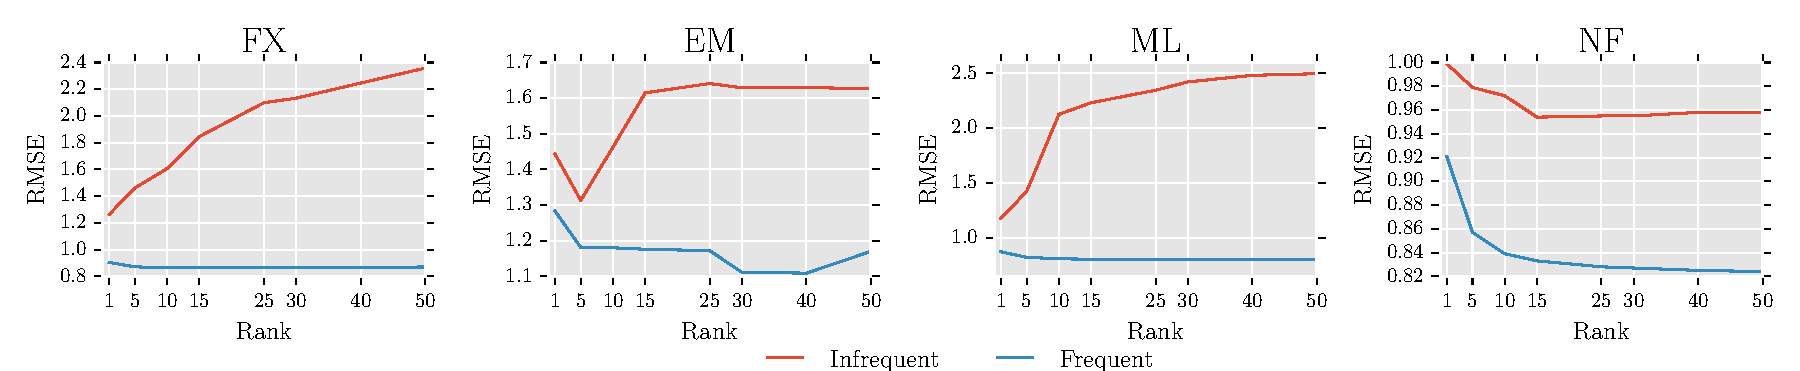
\includegraphics[scale=0.5]{figures/infreq_freq_RMSES.pdf} 
  \caption{Test RMSE of the frequent and infrequent items in real datasets.}
  \label{fig:freq_inFreq_rmse}
\end{figure*}


\begin{figure*}[hbt]
  %\hspace*{-.75cm}
  %\centering
  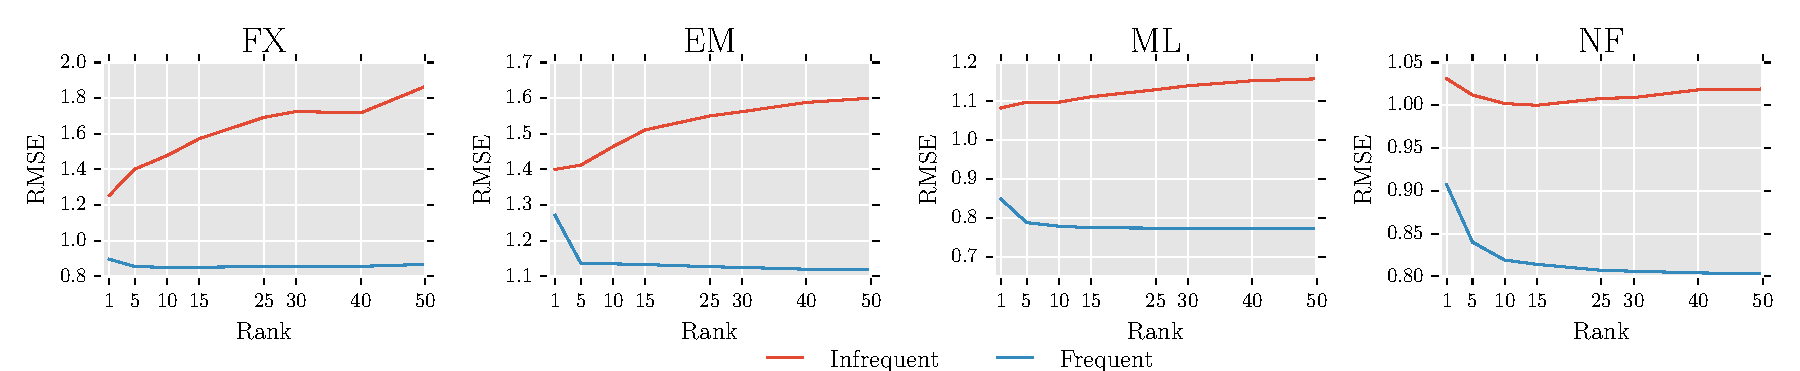
\includegraphics[scale=0.5]{figures/infreq_freq_user_RMSES.pdf} 
  \caption{Test RMSE of the frequent and infrequent users in real datasets.}
  \label{fig:freq_inFreq_user_rmse}
\end{figure*}

\iffalse
\begin{figure*}[hbt]
  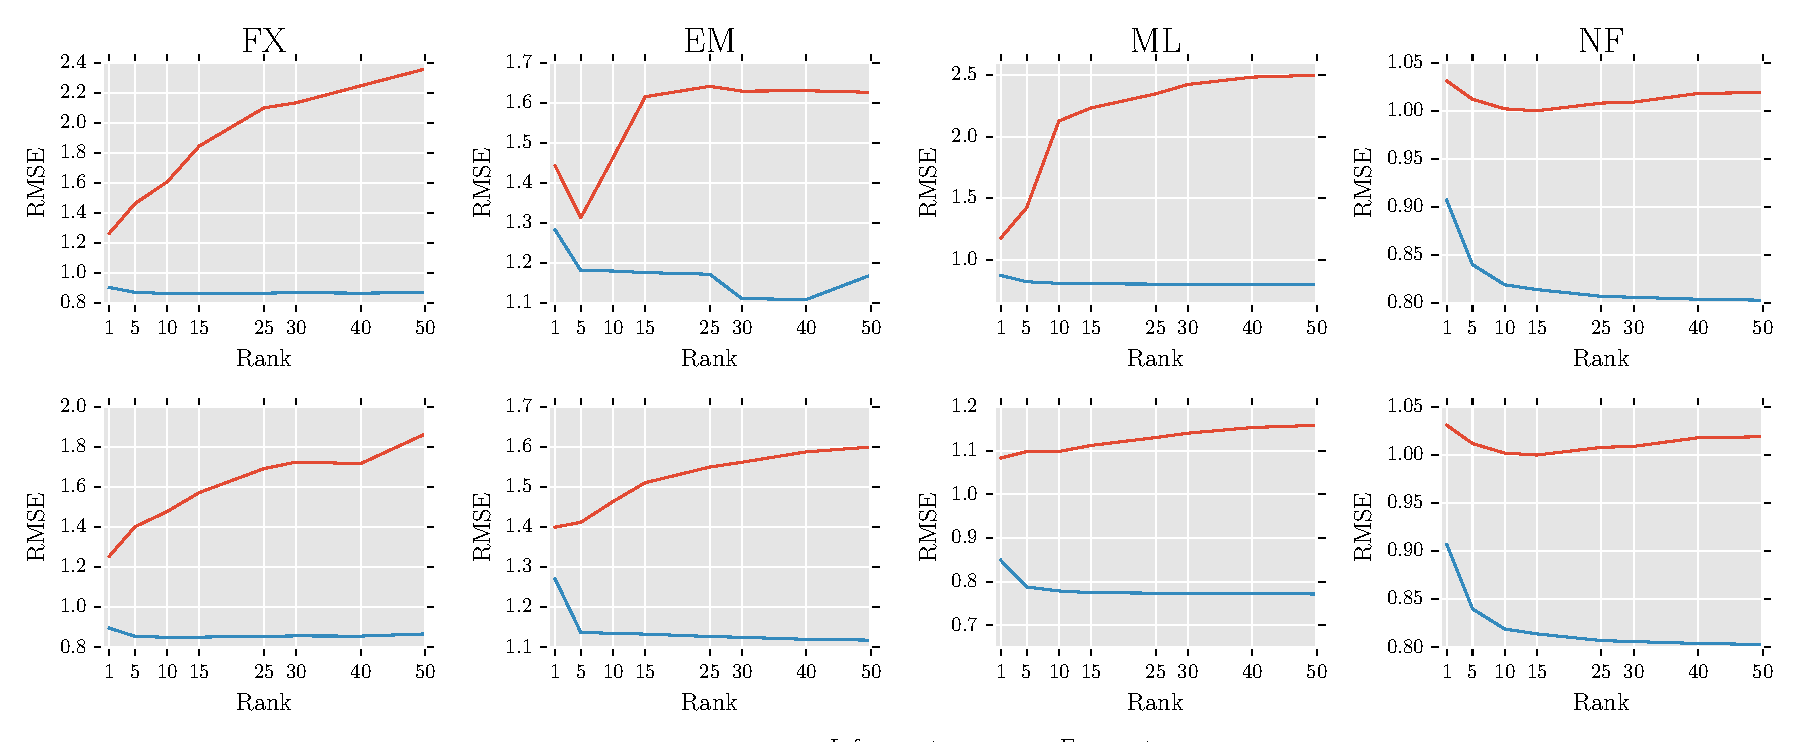
\includegraphics[scale=0.5]{figures/infreq_freq_all_RMSES.pdf} 
  \caption{Test RMSE of the frequent and infrequent users in real datasets.}
  \label{fig:freq_inFreq_all_rmse}
\end{figure*}
\fi

